\part{Microservice Architecture}

\begin{frame}{Cloud Deployment Models – Terminology}
	\begin{figure}
  	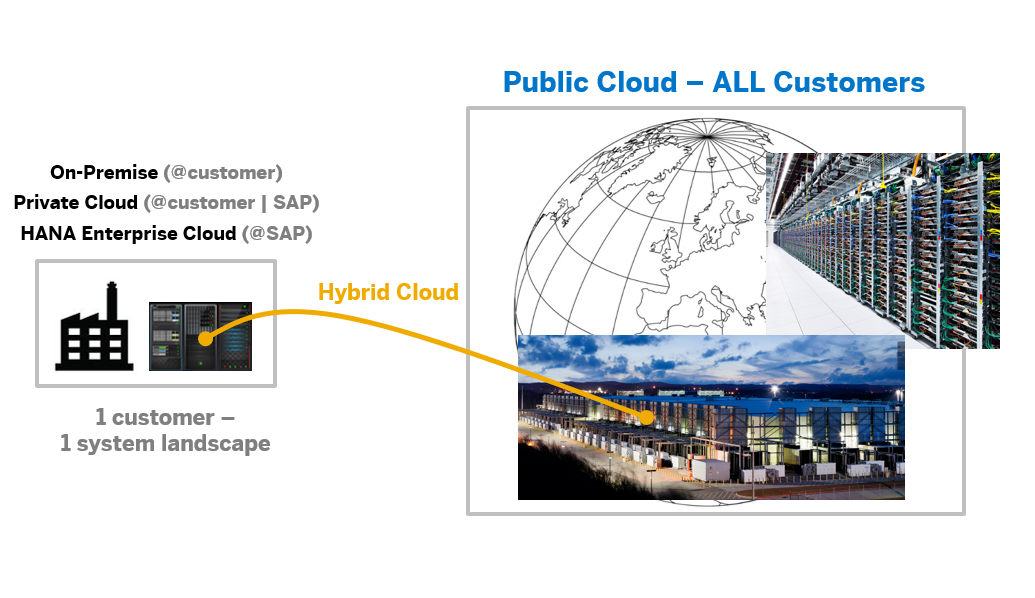
\includegraphics[width=1.0\textwidth]{../MicroServiceArchitecture/images/CloudTerminology}
	\end{figure}
\end{frame}


\begin{frame}{Requirements for a Public Cloud Application}
	\begin{columns}
	\begin{column}{.55\textwidth}
	\begin{itemize}
		\item \textbf{Boundless Scalability}: millions of users, thousands of servers, petabytes of data, globally distributed\\\vspace{9mm}
		\item \textbf{High Availability}: zero downtime deployments, seamless failover\\\vspace{9mm}
		\item \textbf{Fast Innovation}: develop, build and ship in short cycles \emph{within a day}\\\vspace{9mm}
	\end{itemize}
	\end{column}
	\begin{column}{.28\textwidth}
		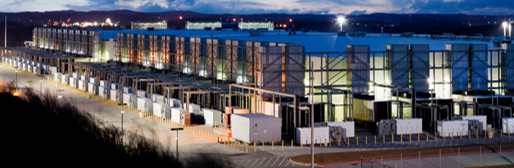
\includegraphics[width=1.2\textwidth]{../MicroServiceArchitecture/images/ComputingCenter}\\
		\vspace{0.3cm}
		
\includegraphics[width=0.7\textwidth]{../MicroServiceArchitecture/images/24-7}\\
		\vspace{0.5cm}
		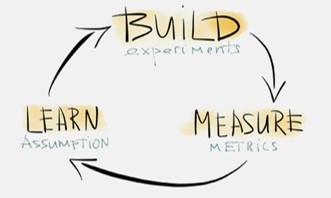
\includegraphics[width=1.2\textwidth]{../MicroServiceArchitecture/images/BuildMeasureLearn}
	\end{column}
	\end{columns}
\end{frame}


\begin{frame}{\large SAP's Traditional Development and Deployment Model}
\textbf{Characteristics of the traditional model}
\begin{itemize}
	\item SAP systems are one logical system with a single (SQL) DB
	\item Transactional consistency for all data is guaranteed
	\item Big, infrequent releases with high risk
\end{itemize}

\vspace{5mm}

\visible<2->{
\textbf{Hard to apply Cloud requirements}
\begin{itemize}
	\item Monolith must be built, tested, deployed and scaled as a whole
	\item Vertical Scaling\footnote{"more expensive servers"} is limited, cost is non-linear
	\item Systems poorly utilized (dev-test, non-peak-times)
	\item High Availability Setup requires almost double the infrastructure
\end{itemize}
}
\end{frame}


\begin{frame}{Microservice Definition}
\begin{quote}
``Microservice architecture is an approach to developing a single \textbf{application} as a \textbf{suite of small services}, each running in its own process and \textbf{communicating with lightweight mechanisms}, often an HTTP REST API. These services are built around \textbf{business capabilities} and \textbf{independently deployable} by \textbf{fully automated deployment} machinery.''
(\colorlink{http://martinfowler.com/articles/microservices.html}{source})
\end{quote}
\centerline{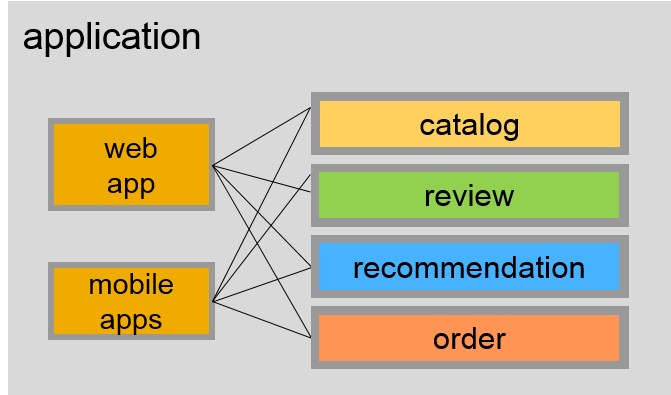
\includegraphics[height=3cm]{../MicroServiceArchitecture/images/MSExample}}
\end{frame}


\begin{frame}{Monolith versus Microservices}
\centerline{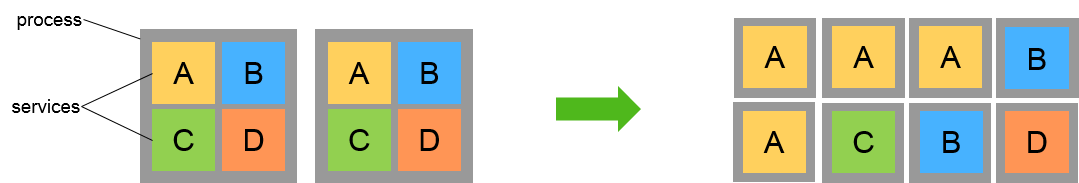
\includegraphics[width=\textwidth]{../MicroServiceArchitecture/images/MS-vs-monolith}}
\vfill
Each Microservice runs in a \textbf{separate process}. This enables \ldots
\begin{itemize}
	\item deploy individually and frequently 
	\item (auto)scale independently to varying loads
\end{itemize}
\end{frame}

\begin{frame}{Independent Evolution} % Technology Heterogeneity
\textbf{You can use technologies \& languages that best fit the problem}\footnote{but be aware of the learning curve and enterprise support}
\begin{itemize}
	\item Microservice is self-contained, i.e. no shared data stores (!)
	\item Using the right tools impacts productivity and performance
\end{itemize}
\vfill
\centerline{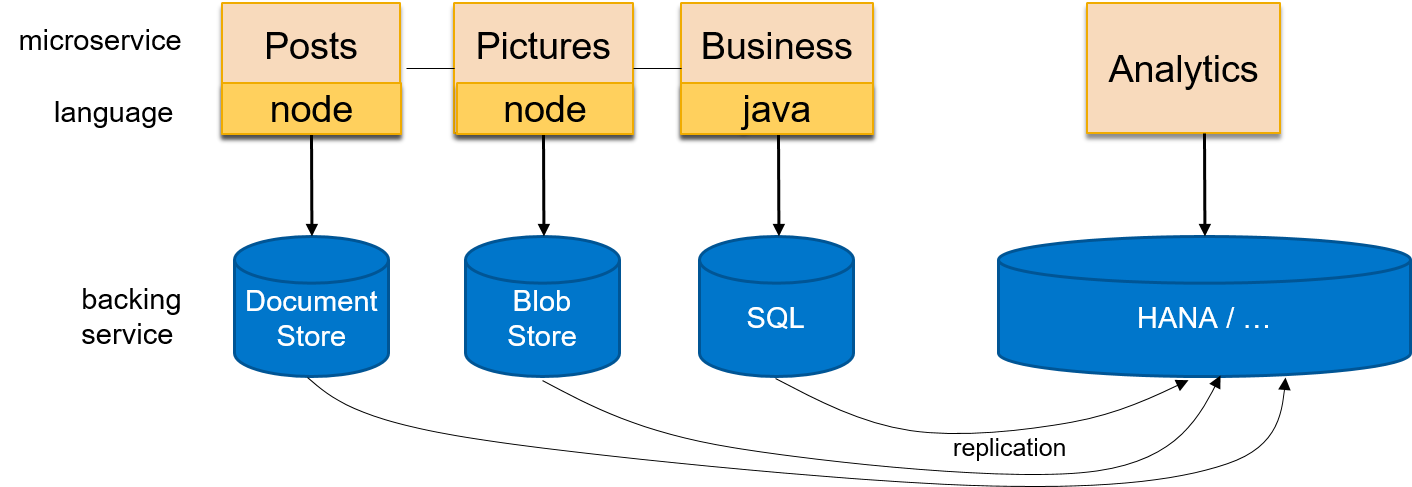
\includegraphics[width=0.7\textwidth]{../MicroServiceArchitecture/images/Polyglot}}
\end{frame}


\begin{frame}{Suitable Service Boundaries}
\begin{columns}[T] 
\begin{column}{.60\textwidth}
\textbf{Microservice is transaction boundary} 
    \begin{itemize}
    \item Service can guarantee data consistency only for local data
    \end{itemize}
\vfill
\textbf{Microservices are loosely coupled} 
    \begin{itemize}
    \item Service should avoid fine-granular and frequent calls to others
    \end{itemize}
\end{column}
\hfill
\begin{column}{.36\textwidth}
\centerline{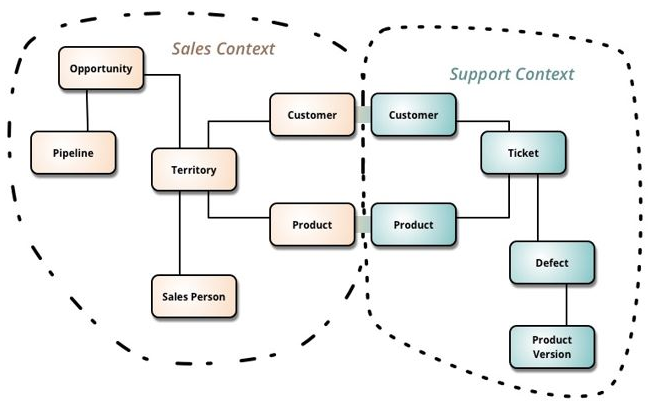
\includegraphics[height=0.42\textheight]{../MicroServiceDesign/images/MicroServiceDesign}}
\end{column}
\end{columns}
\textbf{Start with coarse-grained services}, split later (\colorlink{http://martinfowler.com/bliki/MonolithFirst.html}{source})
    \begin{itemize}
    \item As the logical component boundaries stabilize, break down into finer-grained services as needed for technical / business benefits
    \item Consider \colorlink{https://en.wikipedia.org/wiki/Domain-driven_design}{Domain-Driven-Design}
    \end{itemize}
\end{frame}    


\begin{frame}{Challenges of Distributed Systems}
\textbf{Eventual consistency}
	\begin{itemize}
	\item cross service data consistency not immediately guaranteed
	\end{itemize}

\textbf{Resilience \& isolation of failures}
	\begin{itemize}
	\item Design for failure of all parts (hardware and software)
	\end{itemize}

\textbf{Remote calls over network}
	\begin{itemize}
		\item Network latency, communication overhead
	\end{itemize}

\textbf{Fast Cycles \& Zero Downtime}
	\begin{itemize}
	\item All tests and deployment fully automated
	%\item Features covering multiple microservices still need rollout sync
	\end{itemize}
\end{frame}

\begin{frame}{Business Perspective on Microservices}
The changing structure of business software systems
\begin{itemize}
\item Business software will be a network of applications on an open platform with a strong ecosystem
\item Business applications will be composed of SAP services, partner services and custom developed services
(\colorlink{https://jam4.sapjam.com/profile/06YZ5m1TwB2xKdYPY4UkFv/documents/GywqPwchCFa1CrzQ6GtyJ0}
 {source: SAP Product Strategy 2020})
\end{itemize}
\vfill
\begin{block}{Examples of services:}
	\begin{itemize}
	\item Tax calculation service (SAP offered)
	\item Credit check (by credit card companies), Google Maps integration ...
	\end{itemize}
\end{block}
\end{frame}

\begin{frame}{Summary}
Microservices \ldots
\begin{itemize}
\item are the building blocks of cloud applications
\item implement one concept well (from DB to UI)
\item scale horizontally via processes
\item allow resilience against software and hardware failures
\item can be deployed independently, support continuous delivery
\item can use different technologies
\item raise difficult design topics
\end{itemize}
\end{frame}

\begin{frame}{Further Reading}
\begin{columns}
\begin{column}{.56\textwidth}
\textbf{References}
	\begin{itemize}
	\item \colorlink{https://github.wdf.sap.corp/cc-java-dev/cc-coursematerial/blob/master/MicroServiceArchitecture/Readme.md}{Microservice Notes}
	\item \colorlink{https://jam4.sapjam.com/wiki/show/eBIJTH4EwfD15ymE2nv2pG}{CTO Circle Whitepapers (internal)}
	\item \colorlink{https://jam4.sapjam.com/groups/e7QWGqB0h0ruDy4Ud77aZQ/content?folder_id=VpeQlVtrxiE8uzBIu1lJ9I}{Dragon Blood - Knowledge Sessions}
	\item \colorlink{http://12factor.net}{12 Factors for CF Applications}
	\item \colorlink{https://jam4.sapjam.com/blogs/show/spPIuI94GYS4rtjCPWttrq}{Dev Talk with Martin Fowler}
	\item \colorlink{http://martinfowler.com/articles/microservices.html}{Microservice Article (Fowler)}
	\item \colorlink{http://microservices.io/patterns/microservices.html}{Microservice Architecture pattern}
	\item \colorlink{http://www.infoq.com/articles/microservices-intro}{Microservices for scalability}
	\item \colorlink{http://blog.philipphauer.de/microservices-nutshell-pros-cons/}{Microservices in a Nutshell}
	\colorlink{http://blog.philipphauer.de/microservices-nutshell-pros-cons/}{Pros and Cons}
	\item \colorlink{http://martinfowler.com/bliki/BoundedContext.html}{Bounded Context Design (Fowler)}
	\end{itemize}
\end{column}
\begin{column}{.42\textwidth}
\textbf{Recommended Books}
	
\includegraphics[height=24mm]{../MicroServiceArchitecture/images/buildingMicroservices}
	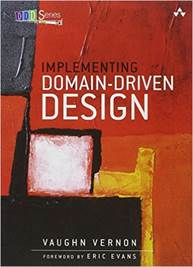
\includegraphics[height=24mm]{../MicroServiceArchitecture/images/implementingDomainDrivenDesign}
\end{column}
\end{columns}
\end{frame}


